\documentclass[a4paper,10pt]{article}
\usepackage{amsmath}
\usepackage{graphicx}
\usepackage{verbatim}
\usepackage[latin1]{inputenc}


% Shortcuts for including equations
\newcommand{\beq}{\begin{equation}}
\newcommand{\eeq}{\end{equation}}
\def\i{\hat{i}}
\def\j{\hat{j}}
\def\k{\hat{k}}

% Document formatting
\setlength{\parindent}{0mm}
\setlength{\parskip}{1.5mm}

% Hyper refs
\usepackage[colorlinks]{hyperref}

\usepackage{listings}
\lstset{language=python}
\lstset{basicstyle=\ttfamily\tiny}
\lstset{frame=single}
\lstset{stringstyle=\ttfamily}
\lstset{keywordstyle=\color{red}\bfseries}
\lstset{commentstyle=\itshape\color{blue}}
\lstset{showspaces=false}
\lstset{showstringspaces=false}
\lstset{showtabs=false}
\lstset{breaklines}
\lstdefinestyle{prt}{frame=none,basicstyle=\ttfamily\small}

\newcounter{subproject}
\renewcommand{\thesubproject}{\alph{subproject}}
\newenvironment{subproj}{
\begin{description}
\item[\refstepcounter{subproject}(\thesubproject)]
}{\end{description}}

%------------------------------------------------------------
\begin{document} 
{\Large\bf Ast1100 Oblig 1}
\newline Thomas Haaland
\section{Problem 7.2}
Skal lande en sonde, Beagle2, p� Mars. Skal beregne veien ned til overflaten.

Det virker to krefter p� sonden. Gravitasjon $\vec{F}_G=G\frac{m_mm_r}{|\vec{r}^3|}\vec{r}$ og friksjon $\vec{f}=-k\vec{v}$. $G$ er newtons gravitasjons konstant, $m_m$ er massen til mars, $m_r$ massen til Beagle2, $\vec{r}$ er posisjonsvektoren fra det ene objektet til det andre, spesielt $\vec{r}=\vec{r}_r-\vec{r}_m$ der $\vec{r}_m$ er posisjonsvektoren til mars og $\vec{r}_r$ posisjonsvektoren til Beagle2, $r=|\vec{r}|$, $k$ er friksjonskoeffisienten og $\vec{v}=\vec{v}_m-\vec{v}_r$ der $\vec{v}_m$ er hastigheten til mars og $\vec{v}_r$ er hastighetsvektoren til Beage2.
\newline
Begge krefter virker p� begge legemer fra det andre legemet, slik at summen av alle krefter er null og alle krefter p� mars er lik alle krefter p� Beagle2: $\Sigma \vec{F}_m = -\Sigma \vec{F}_r$, der $\vec{F}_m$ er krefter p� mars og $\vec{F}_r$ er krefter p� Beagle2. Har her brukt kraft og motkraft, eller Newtons tredje lov. St�r igjen med $\Sigma \vec{F}_m=-\vec{F}_G-\vec{f}$ og $\Sigma \vec{F}_r=\vec{F}_G+\vec{f}$.

Skal l�se bevegelsen til Mars og Beagle2. Bruker Newtons andre lov $\vec{F}=m\vec{a}$
og at $\frac{d^2\vec{x}}{dt}=\vec{a}$. M� dermed l�se 
\newline
\newline
$\int_a^b\frac{d^2\vec{x}}{dt^2}dt=\left[\frac{d\vec{x}}{dt}\right]_a^b$
\newline
\newline
$\int_a^b\frac{d\vec{x}}{dt}dt = \left[\vec{x}\right]_a^b$
\newline
\newline
Denne likningen kan vi l�se generelt numerisk ved Euler-Cromers 
\newline
\newline
$a(t)=\frac{F(t)}{m}$
\newline
$v(t+dt)=v(t)+a(t)dt$
\newline
$x(t+dt)=x(t)+v(t+dt)dt$
\newline
\newline
og gj�r dette for x og y komponentene til vektorfunksjonene $\Sigma \vec{F}_m=m\vec{a}$ og $\Sigma \vec{F}_r=m\vec{a}$. dt er tidsforskjellen mellom hver iterasjon.
Dette kan enkelt skrives inn i et program ved en for- eller while- l�kke: 
\newline
\newline
for i in [0:n]
\newline
$a(i)=\frac{F(i)}{m}$
\newline
$v(i+1)=v(i)+a(i)dt$
\newline
$x(i+1)=x(i)+v(i+1)dt$
\newline
end
\newline
\newline

I koden setter jeg f�rst opp relevante verdier, som initialbetingelser og masse til de forskjellige legemene. I ``Calculation Loop Stuff'' er generelle fysiske konstanter og tall knytta til selve integrasjonsl�kka. I ``Mars'' er verdier knytta spesielt til mars og tilsvarende ``Lander'' knytta til Beagle2.

``Forces'' er en seksjon der kreftene beskrevet over er definert som funksjoner. ``F'' gir kraft som peker fra $r_r$ til $r_m$ som skrevet i programmet. ``f'' gir hastighet som peker motsatt av hastigheten til $v_r$ relativt til $v_m$ som beskrevet i koden.

``Integration Loop'' er en definert funksjon som g�r fra $i=0$ til avstanden mellom $r_r$ og $r_m$ er mindre eller lik mars sin radius. I denne loopen gjenomg�es Euler-Cromer for mars lagt til lister for akselerasjon, hastighet og posisjon, og deretter det samme for Beagle2.

Deretter kommer en seksjon der listene blir reformatert p� en slik m�te at det blir enkelt � plotte dem, for s� � bli plotta.

\section{Problem 7.3}

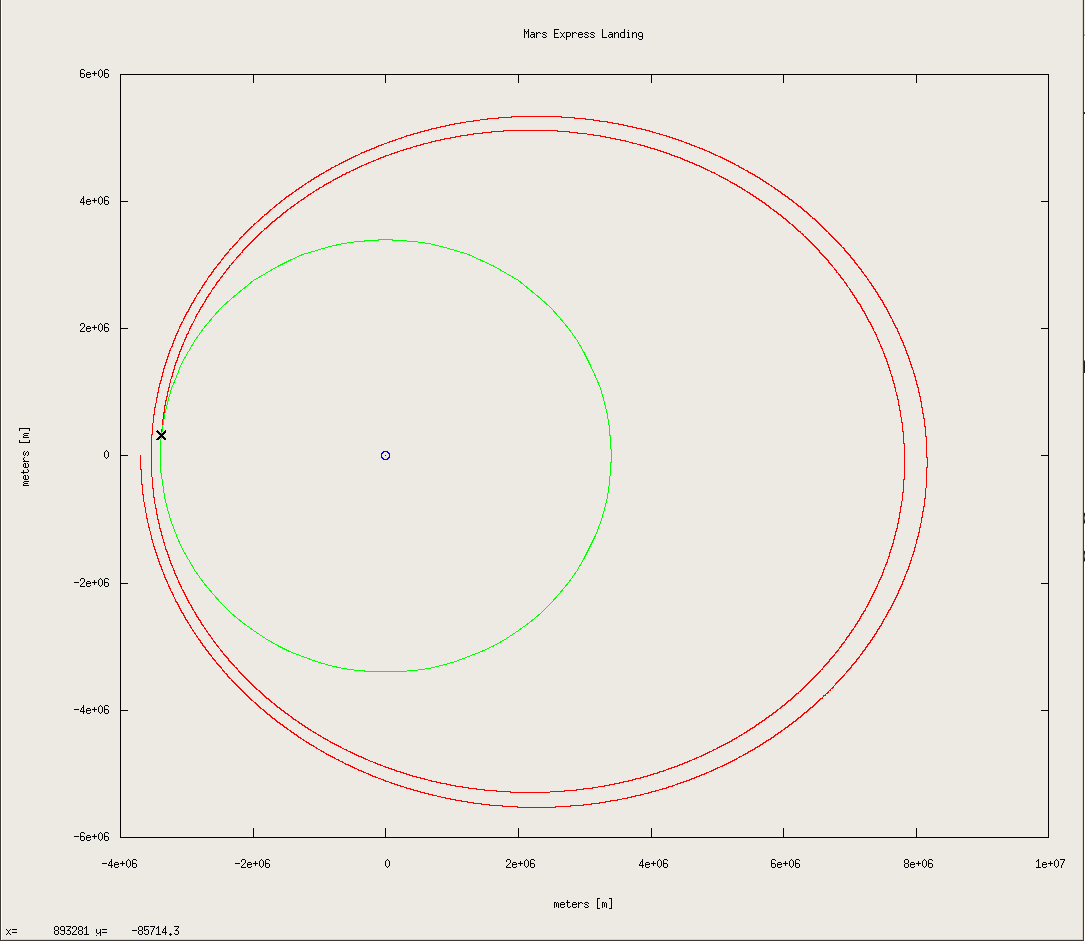
\includegraphics[scale=0.35]{Lander.png}

Ser p� plottet. Nord-s�r aksen g�r langs y-aksen. Ser at Beagle2 lander litt nord for ekvator.

\end{document}
